\documentclass{scrartcl}
\usepackage{color}
\usepackage{url}
\usepackage{cite}
\usepackage{eucal}
\usepackage{fancybox}
\usepackage{amsmath}
\usepackage{epsfig}
\usepackage{amssymb}
\usepackage{amsfonts}
\usepackage{hyperref}
\usepackage{listings}
\usepackage{caption,subcaption}
\usepackage[ruled,vlined]{algorithm2e}
\usepackage{amsmath}
%
\newcommand{\TODO}[1]{\textcolor{red}{\boxed{\mathbf{TODO }} {\textit{#1}} }}
\newcommand{\REMARK}[1]{\textcolor{blue}{\boxed{\mathbf{Remark }} {\textit{#1}} }}
\newcommand{\todo}{\TODO}
\newcommand{\remark}{\REMARK}
\newcommand{\email}[1]{\texttt{#1}}
%
% for algorithms2e
\LinesNumbered
\begin{document}

\title{RNav - R-Tree Navigation Helper on Google App Engine}
\subtitle{CS 764 - Spring 2013 - Innovation Project}

\author{
Aaron Gorenstein\\
	\email{agorenst@cs.wisc.edu}
\and
Rebecca Lam\\
	\email{rjlam@cs.wisc.edu}
\and
Cathrin Weiss\\
	\email{cweiss@cs.wisc.edu}       
}

\date{\today}

\maketitle

%====== OVERVIEW =======================
\section{Overview}
\label{sec:intro}
Google App Engine (GAE) allows for rapid development of web applications without worrying about maintenance or scalability\footnote{\url{https://developers.google.com/appengine/}}. It follows the key-value storage paradigm for persistent as well as in-memory storage. 

We developed a route planning application, \emph{RNav}, that leverages an R-Tree structure on the server side. Using the California Roads data set~\cite{Online:cardata}, we provide route guidance functionality given two input points A and B (assuming A and B are within the described area). The project consists of six components:

\begin{enumerate}
\item The R-Tree data loader, which will convert the geo data into a key-value-compatible R-Tree index (this and part 1 may possibly be combined)
\item The actual R-Tree index, which can process the native R-Tree operations,
\item An algorithm module to compute the shortest route from point A to point B,
\item A simple query engine to process navigation requests, 
\item A query frontend for entering route requests, and
\item A result generator to present the final route to the user. 
\end{enumerate}

Currently Datastore (the GAE key-value store) does not have native support for indexing spatial data and also uses a non-relational database model. Thus, the main challenge for this project was translating the traditional R-Tree implementation in~\cite{DBLP:conf/sigmod/Guttman84} into its GAE equivalent given the constraints of using a key-value store.

The architecture of our project is presented in Section~\ref{sec:architecture} and the implementation details are discussed in Section~\ref{sec:implementation}. 

%====== ARCHITECTURE ==================
\section{Architecture}
\label{sec:architecture}
\begin{figure}[h!]
\begin{center}
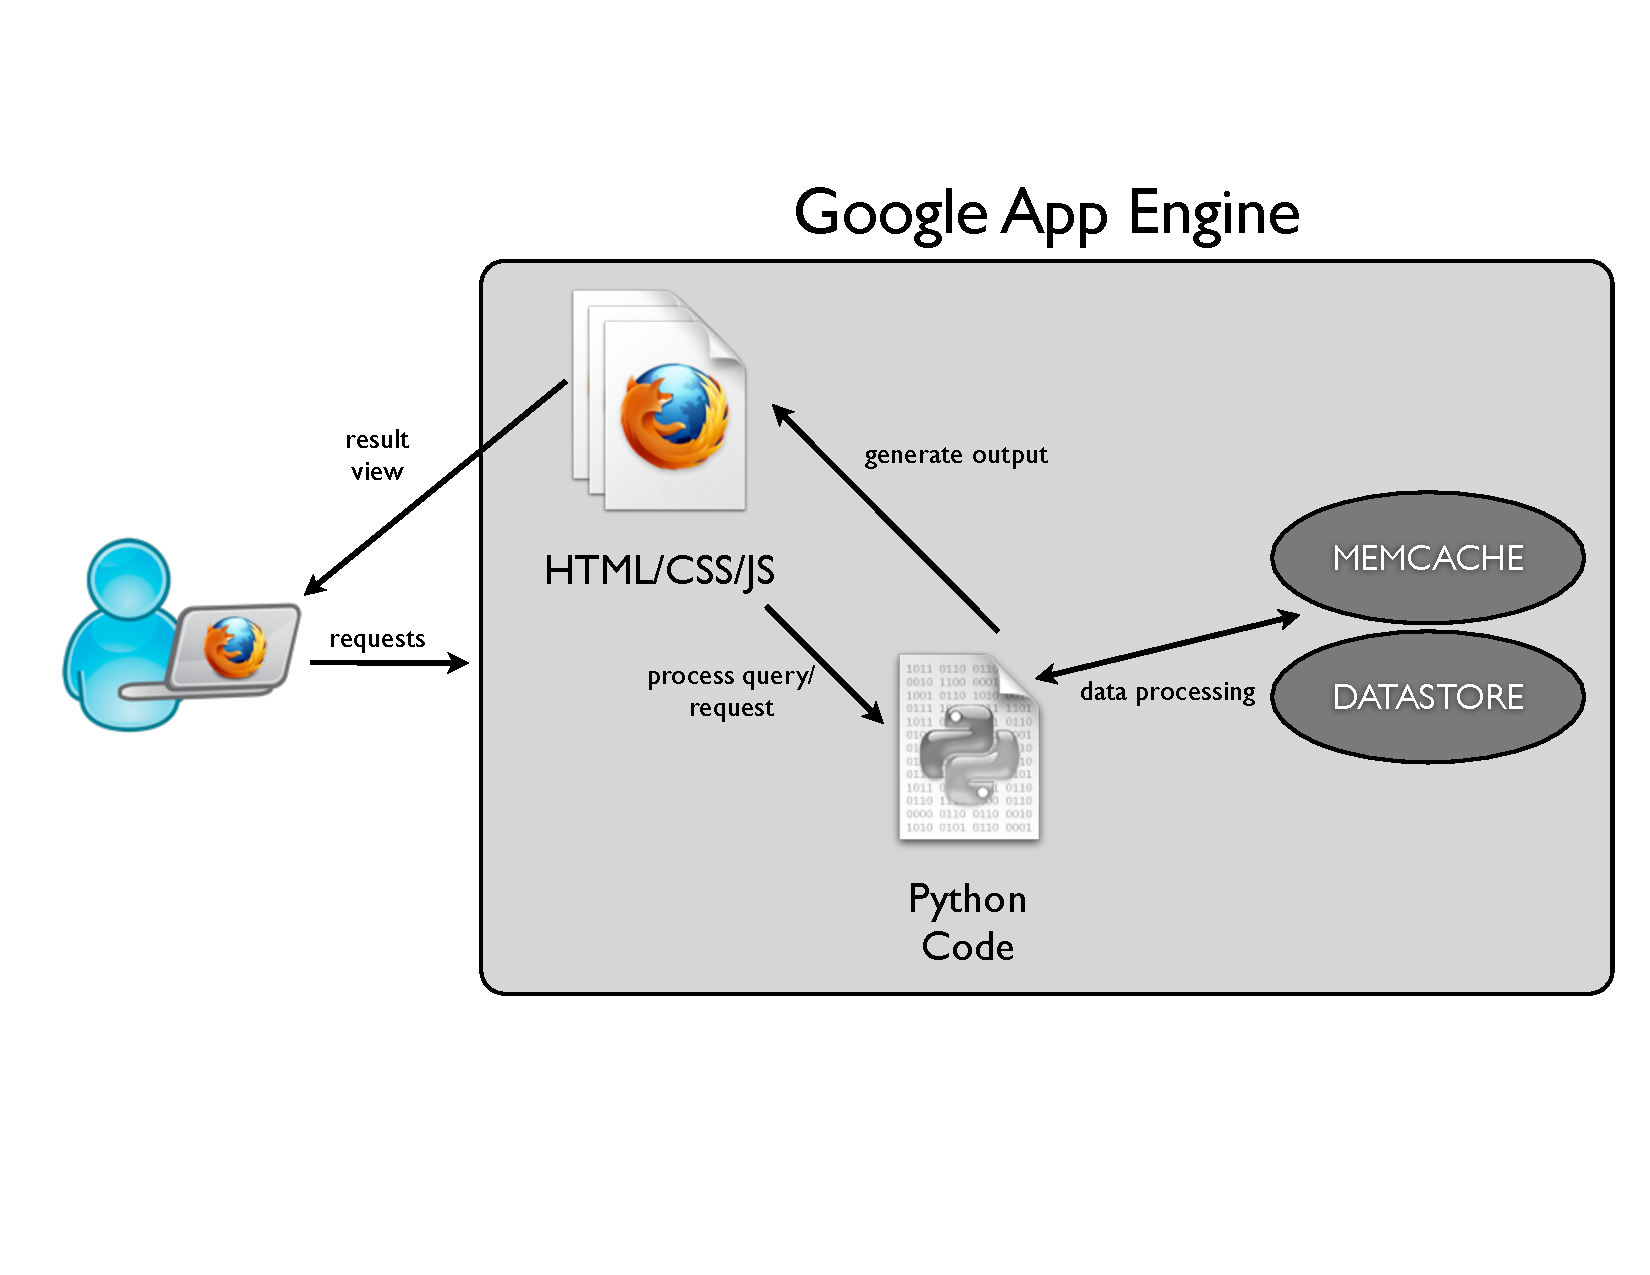
\includegraphics[scale=0.3]{fig/gapps1}
\caption{Google App Engine default architecture}
\label{fig:gappsArch}
\end{center}
\end{figure}

\begin{figure}[h!]
\begin{center}
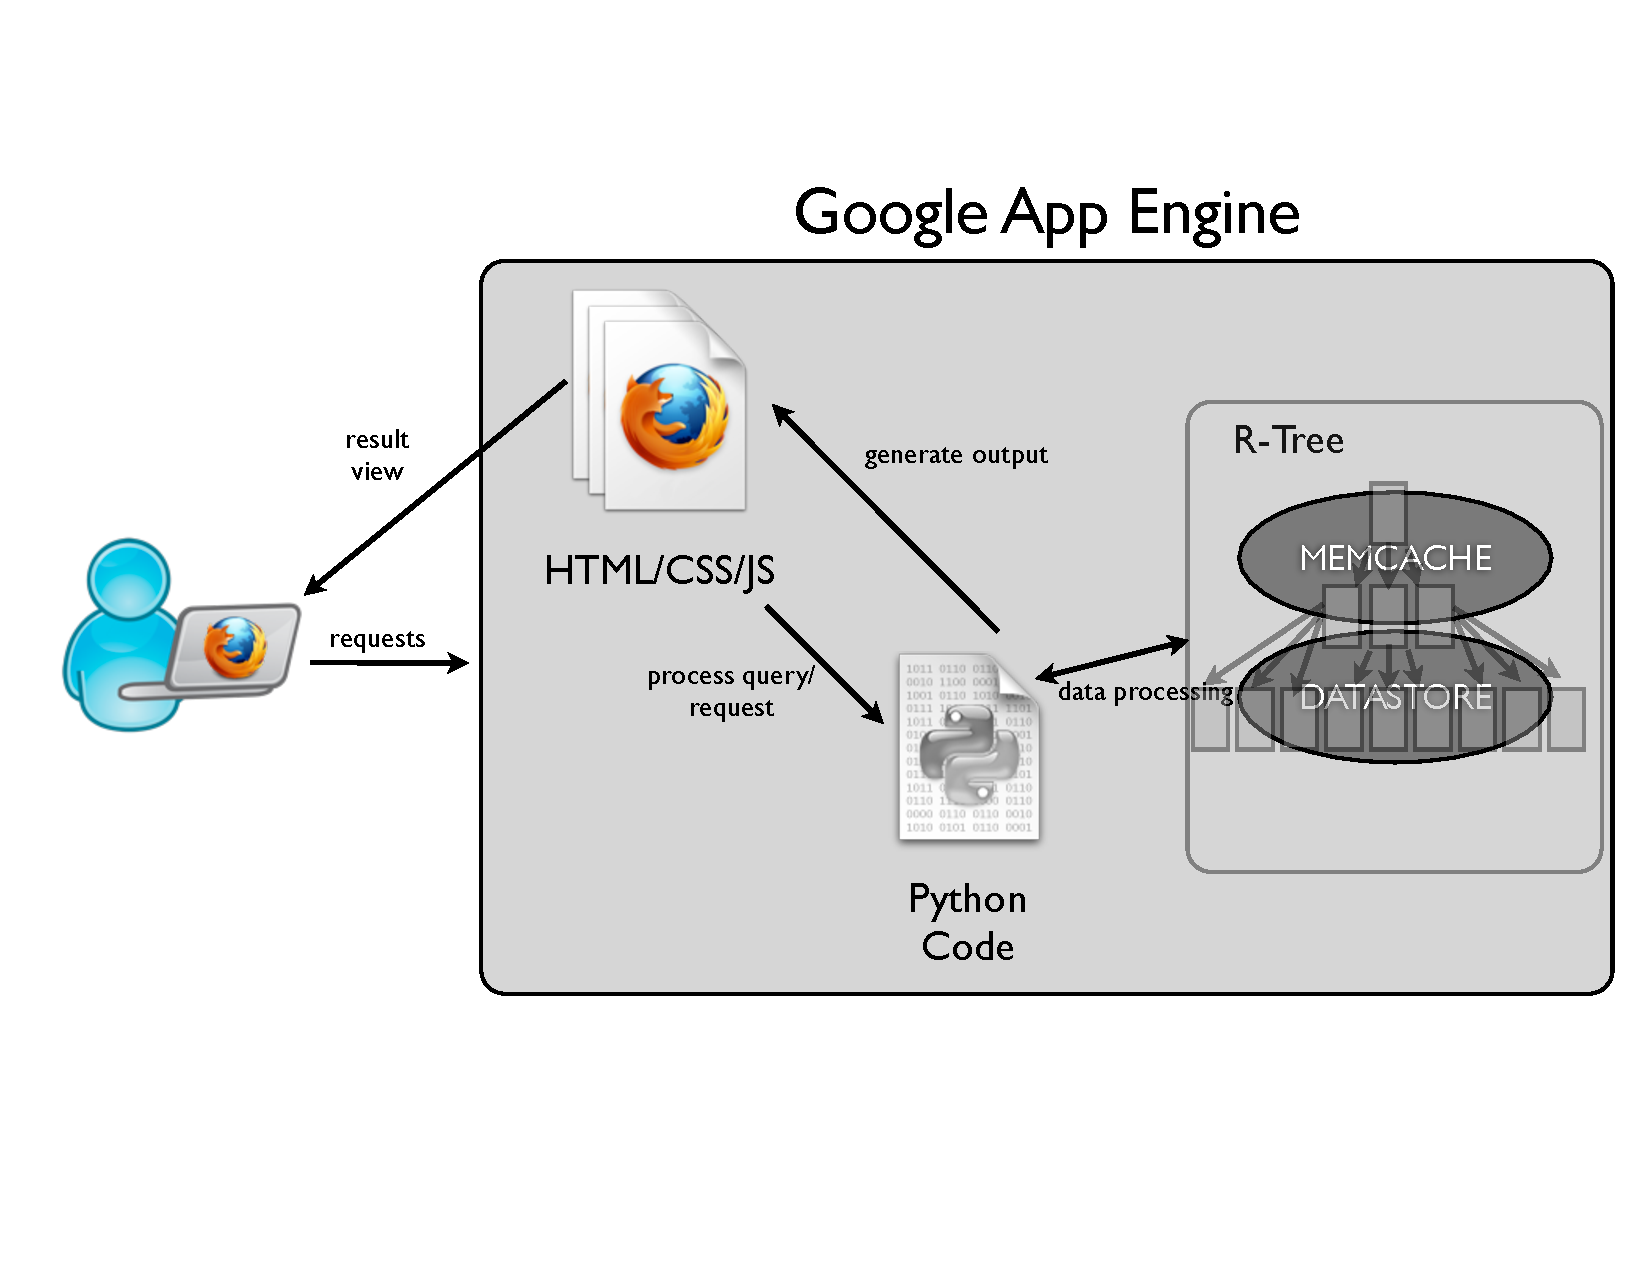
\includegraphics[scale=0.3]{fig/gapps2}
\caption{Google App Engine architecture with R-Tree index}
\label{fig:gappsArch2}
\end{center}
\end{figure}

The architecture of a common Google App Engine application is depicted in Figure~\ref{fig:gappsArch}. A user makes a web request, which gets forwarded to the Python backend, which itself processes the request and interacts with the data store. The data can either be stored persistently or in memory. The latter is referred to as ``Memcache''. Usually data access follows standard key-value protocols. For our project we created an R-Tree index within GAE Datastore to efficiently serve spatial queries. This is schematically shown in Figure~\ref{fig:gappsArch2}. The actual R-Tree layout and implementation is described in Section~\ref{sec:implementation}.

Additionally, we implemented a route-finding algorithm, which takes as input the list of roads retrieved via the R-Tree lookup and generates a route from point A to point B. The resulting is presented to the querying user in a graphical result view.


%====== IMPLEMENTATION ==================
\section{Implementation}
\label{sec:implementation}
\subsection{R-Tree layout in Datastore}
Datastore is a distributed schemaless key-value object datastore that is designed for scalability. It only allows for certain data types to be stored and does not support certain operations such as joins and filtering on multiple attributes. It is possible to store basic data types like integers, short strings, text, and also generic blob data. A Datastore key is composed of a unique identifier and an optional name. When storing an object for the first time, a unique key identifier is automatically created and can be accessed via the Datastore API. 

It is not possible to directly store general objects. Because of this it is not entirely straightforward how to store an R-Tree, which is composed of three non-standard object types: rectangles, entries, and nodes. Recall from Guttman's paper\cite{DBLP:conf/sigmod/Guttman84} that there are two types of nodes in an R-tree: internal and leaf. All nodes have a list of entries describing its children. An internal node entry is of the form ($MBR$, $ptr$) and a leaf node entry is of the form ($MBR$, $oid$), where $MBR$ is the minimum bounding rectangle for child, $ptr$ is a pointer to the child node, and $oid$ is the identifier for the object in the database. In this traditional R-tree, nodes correspond to pages.

In contrast our GAE implementation stores nodes as a key-value pair (key=$key$, value=$entries$), where $key$ is a unique automatically generated value and $entries$ is a list containing data about the node's children. The entries in $entries$ are blob-serialized using Python's \textit{cPickle} module and are of the form ($MBR$, $child\_key$), where $child\_key$ refers to the Datastore object containing the child node. If it is a leaf node, $child\_key$ is \textit{None} for all entries. In order to refer to a child node within an entry, the entry needs to know the node's key identifier in the data store. Thus, the tree must be built bottom up: we must start by allocating leaf-level nodes, then obtaining their corresponding $key$ from the Datastore to update the relevant $child\_key$ in each parent entry. This continue upwards until we reach the root. To keep track of the root of the R-tree, we store an object containing metadata about the structure in the Datastore. This metadata object stores information such as the root key, the page size, and the minimum number of entries per node. By checking whether the metadata is present, we can infer whether there is a tree saved in the data store or not.

Insertion and search are performed as described by Guttman\cite{DBLP:conf/sigmod/Guttman84} except we navigate to different nodes using keys instead of pointers. Our implementation also uses the quadratic split algorithm discussed in the paper on an overflow. Currently we do not have a working delete algorithm, but since our present data set is static it is acceptable. We thus leave the delete function as a future task.

%\TODO{add a descriptive graphic}
% Is this necessary?
% I don't think we actually use memcache?

\subsection{Navigation Algorithm}
We built a small navigation application on top of the R-tree interface.
Given two points, if they are connected by roads, the application returns the list of rectangles which comprise (approximately) the shortest path.
We say approximately because the ``distance'' between two roads is simply the size of the one you're currently on---this design decision was purely due to time and technical limitations.
What were the reasons for developing this particular application?

An immediate motivation is that navigation applications are a well-known, simple spatial query that is rather interesting.
Moreover, shortest-path algorithms (in our case, Dijkstra's) are extremely well-known, but they are not often presented in a distributed setting.
Implementing Dijkstra's ``on top of'' a Google app-engine R-tree was an educative foray into distributed graph queries.
We already know the graph is extremely well-behaved: the data being spatial means that the distance between nodes obeys many nice constraints, such as the triangle inequality (our distance approximation notwithstanding).
Our algorithm can be understood by two subroutines.
The main one, algorithm \ref{alg:findpath}, takes two points, generates an appropriate graph, and then searches the graph for the best path.
The details involved in ``generating an appropriate graph'' are shown in algorithm \ref{alg:buildgraph}.

\begin{algorithm}
\caption{BuildGraph: An algorithm to build a search graph using an R-tree.}\label{alg:buildgraph}
\KwData{An R-Tree $R$ and two leaves $\ell_s$, $\ell_t$.}
\KwResult{A graph $G$ to help compute a path between $\ell_s$, $\ell_t$.}
$M\longleftarrow\text{ComputeMBR}(s,t)$ // $M$ is the minimum bounding rectangle on the leaves\;
$\mathcal S\longleftarrow\text{Search}(R,M)$ // $\mathcal S$ is the set of rectangles touched by $M$\;
$V\longleftarrow\{\ell\mid\ell\in\mathcal S\}$ // Our graph has vertex-set $V$ indexed by each $\ell\in\mathcal S$\;
$E\longleftarrow\{(u,v)\mid \ell_u\cap\ell_v\neq\emptyset\}$ // If two leaves overlap, they are connected in $G$. This can be efficiently computed through $\text{Search}(R,u)$ calls\;
$W$ maps $(u,v)$ to $\text{area}(u)$: that edge has weight equal to the area of the outgoing road\;
\Return $G=(V,E,W)$\;
\end{algorithm}

\begin{algorithm}
\caption{FindPath: Our basic navigation algorithm}\label{alg:findpath}
\KwData{An R-Tree $R$ and two points $s$ and $t$.}
\KwResult{A set of connected roads of least path-weight.}
Let $\ell_s$ be the leaf in $R$ closest to $s$\;
Let $\ell_t$ be the leaf in $R$ closest to $t$\;
$G\longleftarrow\text{BuildGraph}(R,\ell_s,\ell_t)$\;
\Return $\text{Dijkstra}(G,s,t)$\;
\end{algorithm}

As implied by the algorithm, the graph Dijkstra's algorithm uses is implicit in the data, and only made explicit in the small areas our algorithm actually needs.
It can only make the graph explicit by using the R-tree, and it is from that interaction things become interesting.
We have two core observations:

1) Using the R-tree can help trim the portion of the graph Dijkstra's algorithm must traverse.
This allows our algorithm to have a better grasp of how big the graph will actually be, and so may improve performance.
In production applications, the graphs may be so large that a shortest-path algorithm will have to be carefully engineered to handle the giant input.
Here we see that the R-tree allows for a natural ``trimming'' of the input graph, perhaps helping make it more manageable.
The downside is that it may lead to a slightly non-optimal path, if in fact the best roads involve going ``out of our way'' a bit, but due to the nice properties of spatial data it will not be too bad.
In the extreme case, the \emph{only} paths may be very winding and leave the trimmed area, so our search would fail!
We are saving our user a very long drive, however.

2) Using R-trees leads to a natural \emph{partition} of the graph.
Imagine a slight extension to this algorithm, where we wish to record the number of times a road is traversed.
Thus a counter is associated with each road, and to update a path requires a \emph{write lock}.
As we build our graph from the R-tree, this immediately and naturally partitions the graph, so our thread would only have a lock on some small part of the graph, easily expressed by a minimum bounding rectangles.
To our knowledge there is \emph{no such} locking mechanism so simple for graphs.
Perhaps this is a reasonable way to approach concurrent graph access, a notoriously tricky problem.

Even in this simple illustration we have seen that R-trees have very interesting interactions with compelling applications.


% Will we include any tests we performed on this?

\section{Conclusion}
We were able to create RNav, a route planning application built using Google App Engine. It utilizes an R-tree structure built on top of a key-value datastore on the back-end to index data on roads in California. In addition to the R-tree, RNav is comprised of components such as the R-tree loader, navigation algorithm, and front-end. The application is available at \url{http://r-tree.appspot.com}

\bibliographystyle{abbrv}
\bibliography{main}

\end{document}
